\chapter{Análises Realizadas}

	Um dos objetivos do sistema é servir como fonte para futuras pesquisas na área. Para determinar essa possibilidade, foi feita uma análise da base desenvolvida. Essa análise pode ajudar a determinar o melhor modelo de propagação a ser utilizado. Foi avaliada a disponibilidade de canais para o Estado do Rio de Janeiro, ou seja, a quantidade de canais disponíveis para localizações predefinidas do Estado. Foi feita, também, uma análise individual sobre os canais, de forma a determinar quais são os canais que se encontram com maior disponibilidade.

	Essas análises ajudam a identificar a possibilidade de implantação de rádios cognitivos no Rio de Janeiro.

\section{Dataset criado}

Primeiramente foram selecionados pontos distribuídos homogeneamente pelo Estado do Rio de Janeiro.

Para isso, foi criado um retângulo em volta do Estado conforme indicado na figura~\ref{fig:datasetrec}.

\begin{figure}[htb]
\centering
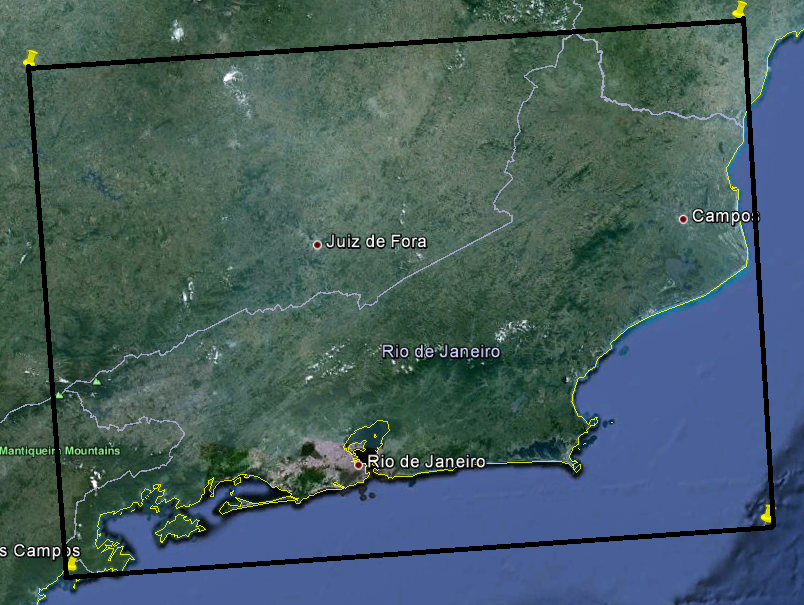
\includegraphics[width=1.0\textwidth]{figs/datasetrec}
\caption[Dataset Utilizado]
{Dataset Utilizado}
\label{fig:datasetrec}
\end{figure} 


\FloatBarrier

Esse retângulo foi percorrido em sua totalidade, variando a latitude e a longitude em 0,01. Para determinar quais desses pontos de fato faziam parte do Rio foi utilizado um serviço online aberto de geolocalização, o GeoNames~\cite{geoloc}.  Foi utilizado o serviço de geocodificação reversa, onde é informado ao sistema um par de coordenadas geográficas e um endereço é recebido como resposta. A partir desse endereço foi identificado a qual Estado o ponto pertencia.

Após se percorrer todo o retângulo foram obtidos 26776 pontos.

\section{Disponibilidade de canais no Rio de Janeiro}

 O sistema desenvolvido foi utilizado para identificar, para cada um dos 26776 pontos, a disponibilidade de canais. Para cada um desses pontos o sistema foi acionado 7 vezes, sempre utilizando um modelo ou parâmetro diferente. 

Para efeito de cálculo, foi considerado para cada ponto calculado um US com potência de 10 W. Esse valor, embora acima dos valores médios indicados no capítulo anterior, apresentou resultados satisfatórios. Esse valor foi escolhido para demonstrar uma situação de pior caso de disponibilidade.

Os seguintes modelos foram utilizados nas buscas:

\begin{itemize}
\item Modelo Free Spaces
\item Modelo Two Ray Ground
\item Modelo Log Distance, utilizando \begin{math}\alpha=2 \end{math}
\item Modelo Log Distance, utilizando \begin{math}\alpha=2,5 \end{math}
\item Modelo Log Distance, utilizando \begin{math}\alpha=3 \end{math}
\item Modelo Log Distance, utilizando \begin{math}\alpha=3,5 \end{math}
\item Modelo Log distance, utilizando \begin{math}\alpha=4 \end{math}
\end{itemize}

Para cada um desses modelos foram plotados histogramas, com informações sobre os canais mais disponíveis, e foram criados mapas de calor utilizando a ferramenta MyHeatMaps~\cite{heatmaps}. Os mapas representam a quantidade de canais disponível por localização. 

Os mapas de calor possuem cores que vão do roxo escuro ao amarelo. O roxo representa localizações onde o número de canais disponíveis é o mínimo identificado, enquanto o amarelo representa áreas onde o número de canais corresponde ao máximo. Cores entre o roxo e o amarelo representam regiões com valores entre o mínimo e o máximo apresentados.

Os canais 63 até 68 foram encontrados como disponíveis em todas as localizações verificadas para todos os modelos. Eles não serão demonstrados nos histogramas por escolha estética.

\subsection{Modelo Free Spaces}

A figura~\ref{fig:histogramafreespaces} representa o histograma de disponibilidade de canais utilizando o modelo Free Space. A figura~\ref{fig:freespacesheatmap} representa o mapa de calor para esse modelo.

\begin{figure}[htb]
\centering
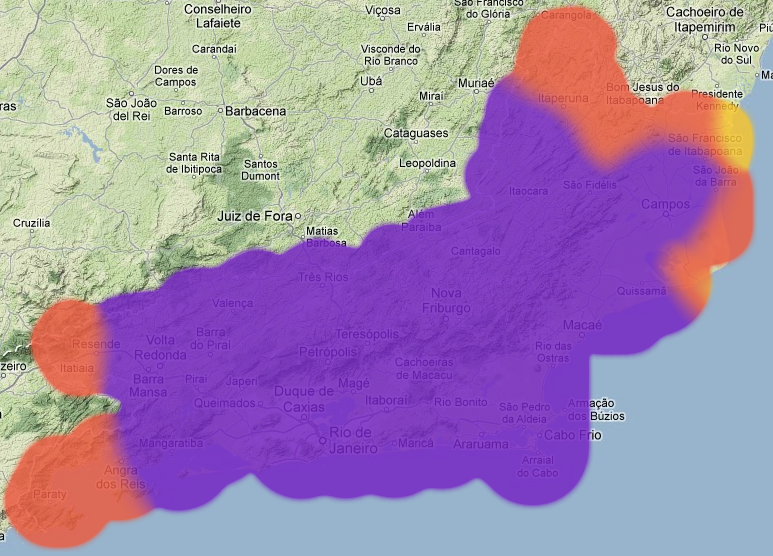
\includegraphics[width=1.0\textwidth]{figs/freespacesheatmap}
\caption[Mapa de calor para o modelo Free Space]
{Mapa de calor para o modelo Free Space}
\label{fig:freespacesheatmap}
\end{figure} 

\begin{figure}[htb]
\centering
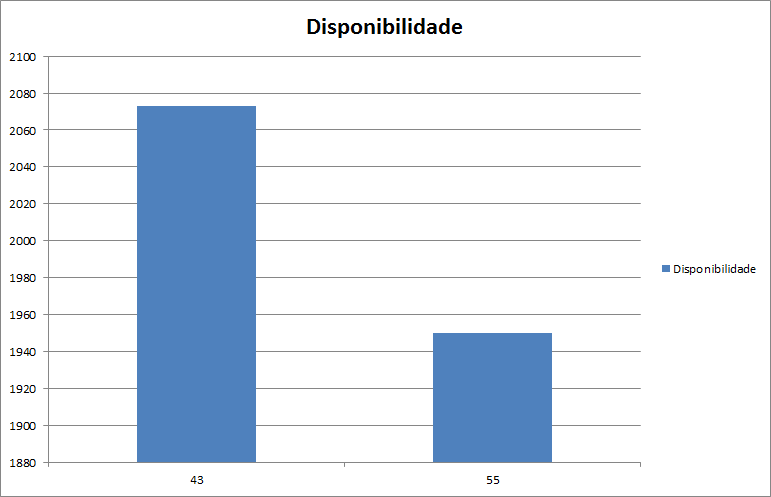
\includegraphics[width=1.0\textwidth]{figs/histogramafreespaces}
\caption[Histograma de disponibilidade de canais para o modelo Free Space]
{Histograma de disponibilidade de canais para o modelo Free Space}
\label{fig:histogramafreespaces}
\end{figure} 


\FloatBarrier

Esse modelo acusou uma média de 8,15 canais disponíveis por localização. Sendo 10 a quantidade máxima de canais disponíveis em uma localização e 8 a mínima.


\subsection{Modelo Two Ray Ground}

A figura~\ref{fig:histogramatworay} representa o histograma de disponibilidade de canais utilizando o modelo Two Ray Ground. A figura~\ref{fig:tworayheatmap} representa o mapa de calor para esse modelo.

\begin{figure}[htb]
\centering
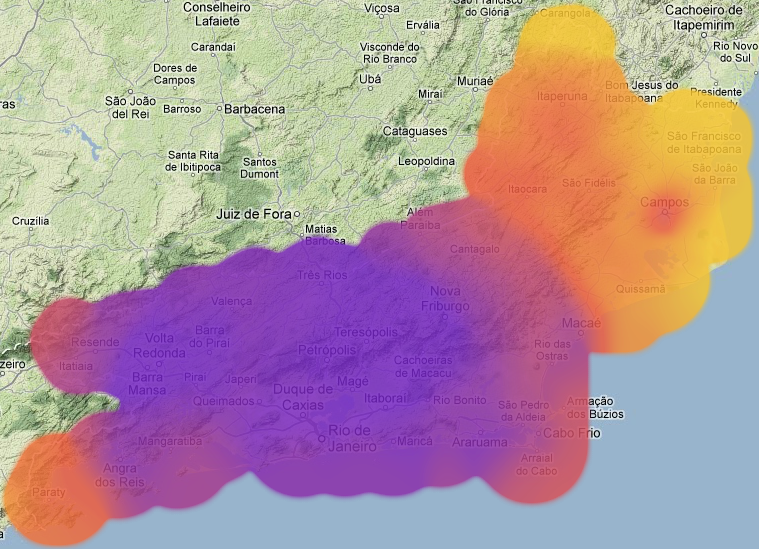
\includegraphics[width=1.0\textwidth]{figs/tworayheatmap}
\caption[Mapa de calor para o modelo Two Ray Ground]
{Mapa de calor para o modelo Two ray Ground}
\label{fig:tworayheatmap}
\end{figure} 

\begin{figure}[htb]
\centering
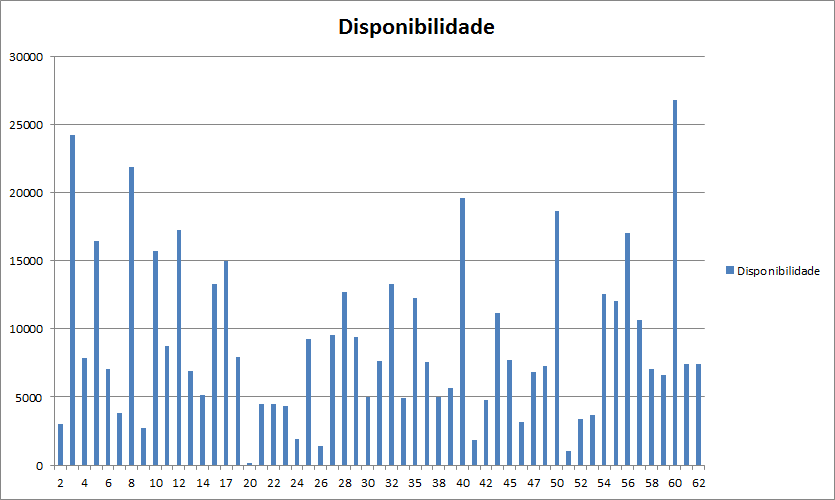
\includegraphics[width=1.0\textwidth]{figs/histogramatworay}
\caption[Histograma de disponibilidade de canais para o modelo Two Ray Ground]
{Histograma de disponibilidade de canais para o modelo Two Ray Ground}
\label{fig:histogramatworay}
\end{figure} 


\FloatBarrier

Esse modelo acusou uma média de 25,38 canais disponíveis por localização. Sendo 60 a quantidade máxima de canais disponíveis em uma localização e 10 a mínima.

\subsection{Modelo Log Distance}

Para analisar a capacidade de indicar parâmetros ao sistema, a constante de decaimento \begin{math}\alpha \end{math} foi alternada entre alguns valores diferentes.

\subsubsection{Constante = 2}

A figura~\ref{fig:histogramalogdist2} representa o histograma de disponibilidade de canais utilizando o modelo Log Distance usando \begin{math}\alpha=2 \end{math}. A figura~\ref{fig:LogDist2heatmap} representa o mapa de calor para esse modelo.

\begin{figure}[htb]
\centering
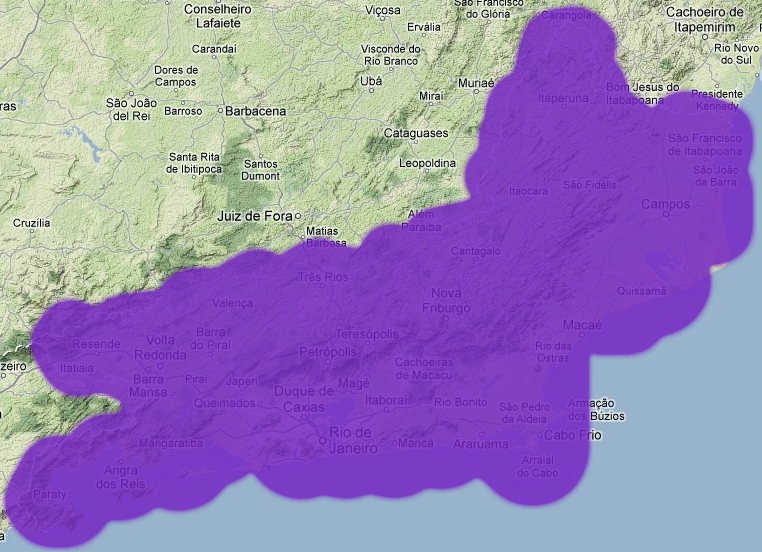
\includegraphics[width=1.0\textwidth]{figs/logdist2heatmap}
\caption[Mapa de calor para o modelo Log Distance usando 2 como constante de decaimento]
{Mapa de calor para o modelo Log Distance usando 2 como constante de decaimento}
\label{fig:LogDist2heatmap}
\end{figure} 

\begin{figure}[htb]
\centering
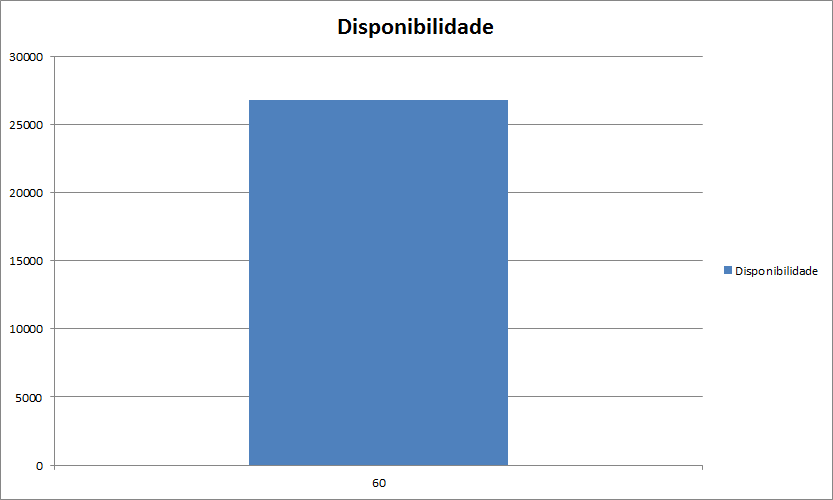
\includegraphics[width=1.0\textwidth]{figs/histogramalogdist2}
\caption[Histograma de disponibilidade de canais para o modelo Log Distance usando 2 como constante de decaimento]
{Histograma de disponibilidade de canais para o modelo Log Distance usando 2 como constante de decaimento}
\label{fig:histogramalogdist2}
\end{figure} 


\FloatBarrier

Esse modelo acusou uma média de 8 canais disponíveis por localização. Sendo 8 a quantidade máxima de canais disponíveis em uma localização e 8 a mínima.

\subsubsection{Constante = 2,5}

A figura~\ref{fig:histogramalogdist25} representa o histograma de disponibilidade de canais utilizando o modelo Log Distance usando \begin{math}\alpha=2,5 \end{math}. A figura~\ref{fig:LogDist25heatmap} representa o mapa de calor para esse modelo.

\begin{figure}[htb]
\centering
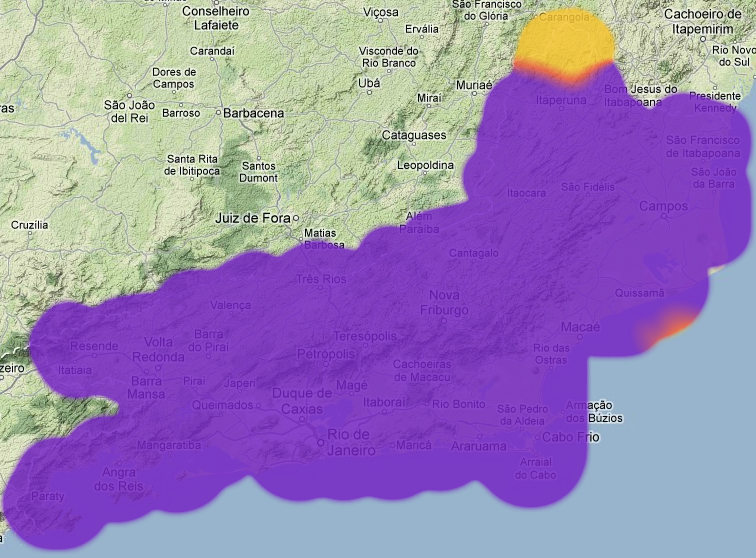
\includegraphics[width=1.0\textwidth]{figs/logdist25heatmap}
\caption[Mapa de calor para o modelo Log Distance usando 2,5 como constante de decaimento]
{Mapa de calor para o modelo Log Distance usando 2,5 como constante de decaimento}
\label{fig:LogDist25heatmap}
\end{figure} 

\begin{figure}[htb]
\centering
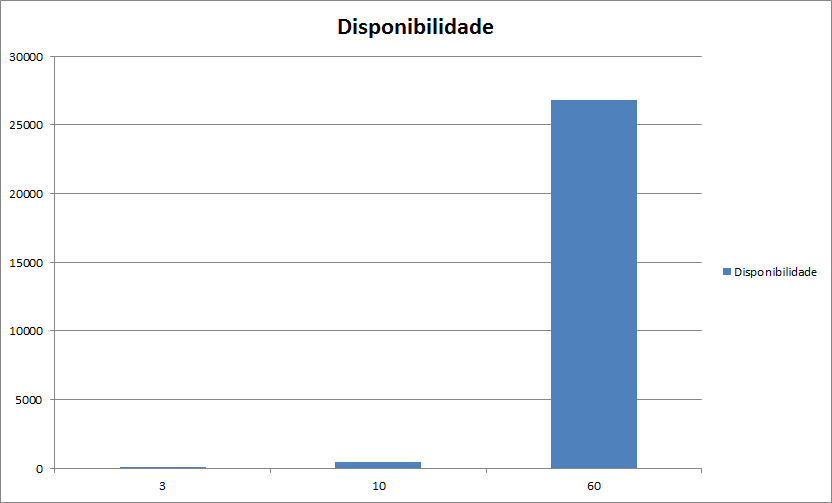
\includegraphics[width=1.0\textwidth]{figs/histogramalogdist25}
\caption[Histograma de disponibilidade de canais para o modelo Log Distance usando 2,5 como constante de decaimento]
{Histograma de disponibilidade de canais para o modelo Log Distance usando 2,5 como constante de decaimento}
\label{fig:histogramalogdist25}
\end{figure} 

\FloatBarrier

Esse modelo acusou uma média de 8,01 canais disponíveis por localização. Sendo 9 a quantidade máxima de canais disponíveis em uma localização e 8 a mínima.

\subsubsection{Constante = 3}

A figura~\ref{fig:histogramalogdist3} representa o histograma de disponibilidade de canais utilizando o modelo Log Distance usando \begin{math}\alpha=3 \end{math}. A figura~\ref{fig:LogDist3heatmap} representa o mapa de calor para esse modelo.

\begin{figure}[htb]
\centering
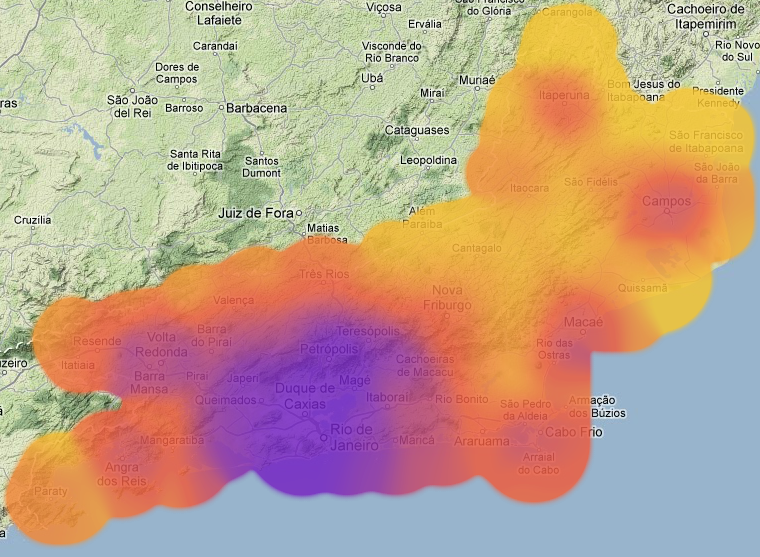
\includegraphics[width=1.0\textwidth]{figs/logdist3heatmap}
\caption[Mapa de calor para o modelo Log Distance usando 3 como constante de decaimento]
{Mapa de calor para o modelo Log Distance usando 3 como constante de decaimento }
\label{fig:LogDist3heatmap}
\end{figure} 

\begin{figure}[htb]
\centering
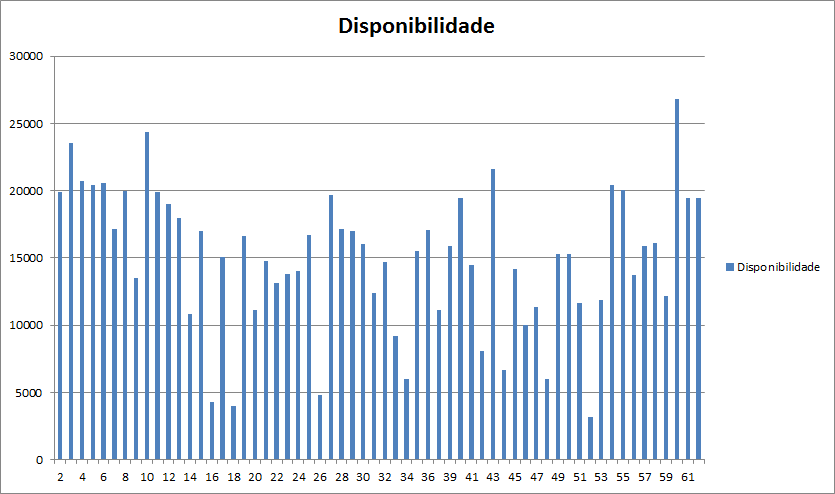
\includegraphics[width=1.0\textwidth]{figs/histogramalogdist3}
\caption[Histograma de disponibilidade de canais para o modelo Log Distance usando 3 como constante de decaimento]
{Histograma de disponibilidade de canais para o modelo Log Distance usando 3 como constante de decaimento}
\label{fig:histogramalogdist3}
\end{figure} 

\FloatBarrier

Esse modelo acusou uma média de 40,52 canais disponíveis por localização. Sendo 67 a quantidade máxima de canais disponíveis em uma localização e 12 a mínima.

\subsubsection{Constante = 3,5}

A figura~\ref{fig:histogramalogdist35} representa o histograma de disponibilidade de canais utilizando o modelo Log Distance usando \begin{math}\alpha=3,5 \end{math}. A figura~\ref{fig:LogDist35heatmap} representa o mapa de calor para esse modelo.

\begin{figure}[htb]
\centering
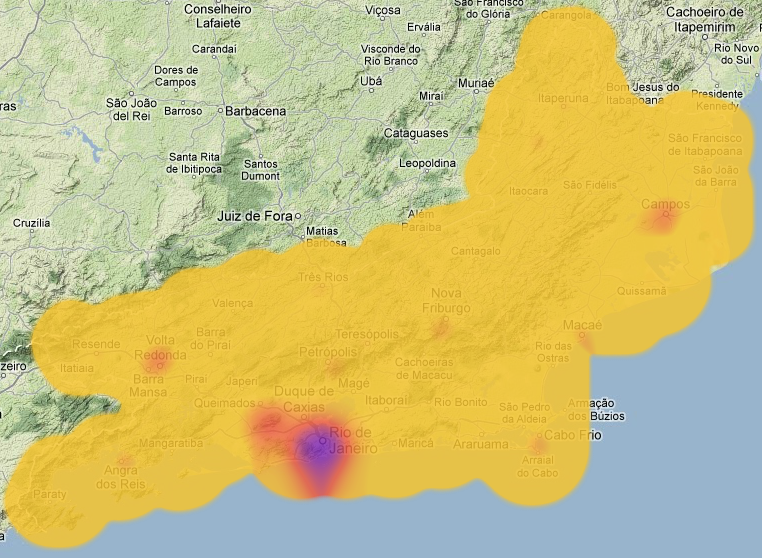
\includegraphics[width=1.0\textwidth]{figs/logdist35heatmap}
\caption[Mapa de calor para o modelo Log Distance usando 3,5 como constante de decaimento]
{Mapa de calor para o modelo Log Distance usando 3,5 como constante de decaimento }
\label{fig:LogDist35heatmap}
\end{figure} 

\begin{figure}[htb]
\centering
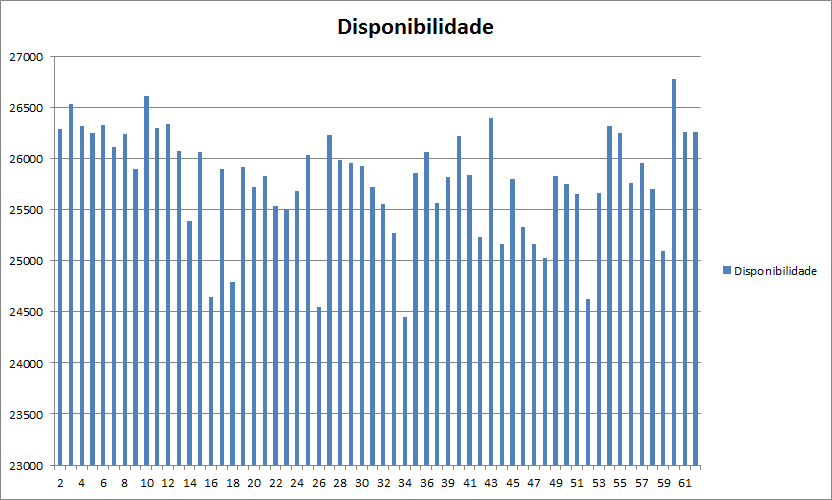
\includegraphics[width=1.0\textwidth]{figs/histogramalogdist35}
\caption[Histograma de disponibilidade de canais para o modelo Log Distance usando 3,5 como constante de decaimento]
{Histograma de disponibilidade de canais para o modelo Log Distance usando 3,5 como constante de decaimento}
\label{fig:histogramalogdist35}
\end{figure} 


\FloatBarrier

Esse modelo acusou uma média de 64,78 canais disponíveis por localização. Sendo 67 a quantidade máxima de canais disponíveis em uma localização e 22 a mínima.

\subsubsection{Constante = 4}

A figura~\ref{fig:histogramalogdist4} representa o histograma de disponibilidade de canais utilizando o modelo Log Distance usando \begin{math}\alpha= 4 \end{math}. A figura~\ref{fig:LogDist4heatmap} representa o mapa de calor para esse modelo.

\begin{figure}[htb]
\centering
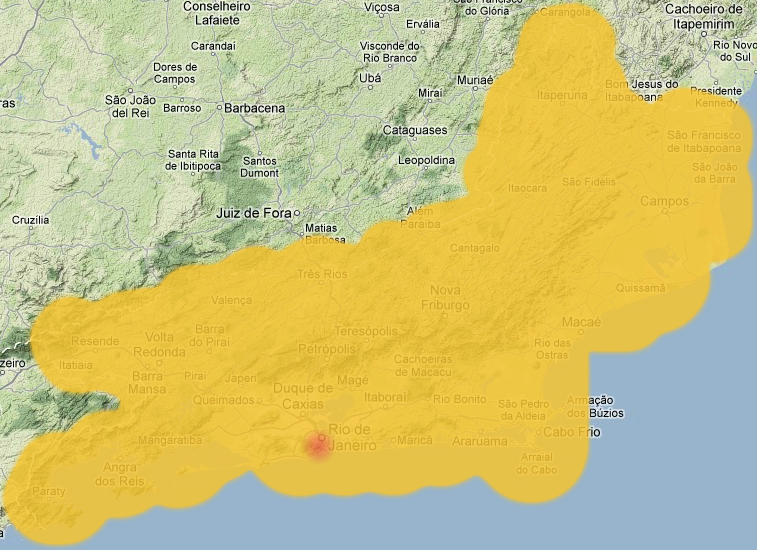
\includegraphics[width=1.0\textwidth]{figs/logdist4heatmap}
\caption[Mapa de calor para o modelo Log Distance usando 4 como constante de decaimento]
{Mapa de calor para o modelo Log Distance usando 4 como constante de decaimento }
\label{fig:LogDist4heatmap}
\end{figure} 

\begin{figure}[htb]
\centering
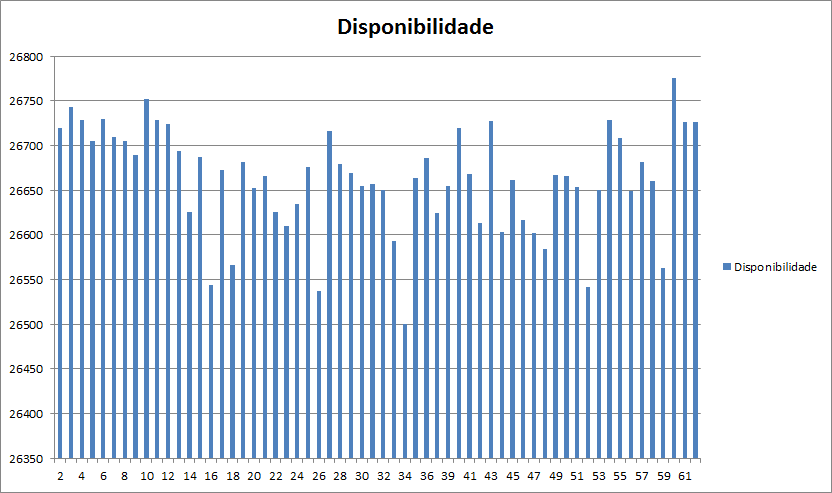
\includegraphics[width=1.0\textwidth]{figs/histogramalogdist4}
\caption[Histograma de disponibilidade de canais para o modelo Log Distance usando 4 como constante de decaimento]
{Histograma de disponibilidade de canais para o modelo Log Distance usando 4 como constante de decaimento}
\label{fig:histogramalogdist4}
\end{figure} 


\FloatBarrier

Esse modelo acusou uma média de 66,75 canais disponíveis por localização. Sendo 67 a quantidade máxima de canais disponíveis em uma localização e 26 a mínima.


\section{Resultado da análise}

\subsection{Diferença entre Modelos}

Como pode ser observado, a diferença de um modelo de propagação para o outro é significativa. É importante que o modelo utilizado pela base seja o mais preciso possível.

Caso o modelo seja muito sensível, ou seja, se o alcance calculado das antenas pelo modelo for muito maior que o alcance real, estará ocorrendo um desperdício. O objetivo dos rádios cognitivos, como mencionado no primeiro capítulo, é aproveitar o espectro de frequência reservado para um dispositivo primário que não está sendo utilizado. Se a base determinar um alcance maior que o real, canais que poderiam estar sendo utilizados serão considerados como ocupados.

No entanto, um modelo pouco sensível também não é bom. Caso um modelo determine alcances menores que os reais, um dispositivo secundário pode acabar escolhendo um canal que já esteja em uso por um primário. Isso acarreta uma condição de interferência entre os dispositivos. É imprescindível que essa interferência não ocorra. Um dispositivo primário tem o direito de utilizar aquele canal, que foi obtido por uma licitação, e tem prioridade total sobre os secundários.

O modelo ideal, portanto, não pode ser muito sensível, nem pouco sensível demais. É mais sensato, para a BDWS, escolher um modelo um pouco mais sensível que o ideal. Embora o desperdício possa existir, seria uma maneira de evitar a interferência entre dispositivos.

\subsubsection{Modelo Free Space}

O Free Space foi o modelo mais sensível entre os utilizados. Ao utilizá-lo, são encontrados valores muito grandes para o alcance das antenas, de forma que, analisando os mapas de calor, todo o espectro de frequência se encontra ocupado no Estado do Rio de Janeiro.

 Ele não pode ser utilizado por uma BDWS, e foi implementado apenas por motivos acadêmicos.

\subsubsection{Two Ray}

O Two Ray é um pouco menos sensível que o Free Space. Os alcances das antenas calculadas por ele já são mais próximos da realidade. Os mapas de calor já apresentam um panorama mais próximo do esperado. Pode-se verificar que as regiões metropolitanas apresentam um espectro de frequência todo ocupado, enquanto que o campo apresenta regiões onde ele está todo disponível.

Esse modelo poderia ser utilizado por uma WSBD. Por prever um alcance um pouco maior que o normal é praticamente garantido que um dispositivo secundário não irá interferir com um primário. No entanto, inevitavelmente, vai desperdiçar algum canal.

\subsubsection{Log Distance}

Foram encontrados resultados bem distintos ao variar o valor da constante de decaimento \begin{math}\alpha \end{math}.

Ao utilizar a constante com valores 2 e 2,5, o modelo se aproxima bastante do Free Space. Assim, ele apresenta as mesmas falhas.

Já ao utilizar a constante com valor 3, o modelo chegou o mais próximo do ideal. Analisando o mapa de calor fica bem evidente a diferença na disponibilidade de canais entre regiões mais e menos povoadas. Os alcances calculados para as antenas se assemelharam a valores reais. Esse modelo foi definido como sendo padrão para a base.

No entanto, ao utilizar a constante com valores 3,5 e 4, o modelo apresentou resultados muito pouco sensíveis. Certamente, os alcances calculados são muito menores que os reais. Isso fica visível nos mapas de calor. A região com baixa disponibilidade de canais se restringe a área próximas de grupos de antenas. Se utilizado por uma BDWS esse modelo pode acabar fazendo com que os dispositivos se encontrem em posição de interferência. Por conta desses motivos, a constante não pode assumir esses valores.

\subsection{Conclusão}

Entre os modelos implementados, o Log Distance, com \begin{math}\alpha=3 \end{math} apresentou os melhores resultados. Como esperado, regiões metropolitanas estão com um grau de disponibilidade de canais muito baixo, já que grande maioria já está sendo utilizado por um dispositivo primário, enquanto que áreas campestres apresentam um grau de disponibilidade maior. Os resultados obtidos confirmam a escolha desse modelo como padrão para a BDWS desenvolvida.

Embora o modelo tenha sido considerado como o ideal entre os estudados não se deve tomá-lo como o mais completo. É ideal que seja implementado um modelo mais completo, que utilize informações como o relevo do terreno e densidade de estruturas, de forma a sempre calcular o alcance dos dispositivos primário com maior precisão.

De maneira geral foi verificado que o Rio de Janeiro é uma área propícia para a implantação de rádios cognitivos. Embora as regiões metropolitanas já estejam densamente utilizadas, foi identificado que em áreas menos povoadas a quantidade de canais disponível é alta.
